% ============================================================
%  VoltGuard — Project Report
%  EGS 2025/2026 — Grupo 4 — Universidade de Aveiro / DETI
% ============================================================
\documentclass[12pt,a4paper,oneside]{report}

% ── Packages ────────────────────────────────────────────────
\usepackage[T1]{fontenc}
\usepackage[utf8]{inputenc}
\usepackage[english]{babel} 
\usepackage[a4paper, top=2.5cm, bottom=2.5cm, left=3cm, right=2.5cm]{geometry}
\usepackage{graphicx}
\usepackage{xcolor}
\usepackage{hyperref}
\usepackage{listings}
\usepackage{booktabs}
\usepackage{longtable}
\usepackage{array}
\usepackage{tabularx}
\usepackage{fancyhdr}
\usepackage{titlesec}
\usepackage{caption}
\usepackage{subcaption}
\usepackage{float}
\usepackage{parskip}
\usepackage{microtype}
\usepackage{lmodern}
\setlength{\emergencystretch}{3em}
\widowpenalty=10000
\clubpenalty=10000
\usepackage{enumitem}
\usepackage{mdframed}
\usepackage{tikz}
\usetikzlibrary{shapes.geometric, arrows.meta, positioning, fit}

% ── Colours ─────────────────────────────────────────────────
\definecolor{voltgreen}{RGB}{34, 139, 34}
\definecolor{voltyellow}{RGB}{255, 193, 7}
\definecolor{codebg}{RGB}{245, 245, 245}
\definecolor{codeframe}{RGB}{200, 200, 200}
\definecolor{primary}{RGB}{30, 80, 160}

% ── Hyperref setup ──────────────────────────────────────────
\hypersetup{
    colorlinks=true,
    linkcolor=primary,
    urlcolor=primary,
    citecolor=primary,
    pdftitle={VoltGuard -- Project Report},
    pdfauthor={Grupo 4 -- EGS 2025/2026},
}

% ── Code listings ───────────────────────────────────────────
\lstset{
    backgroundcolor=\color{codebg},
    frame=single,
    rulecolor=\color{codeframe},
    basicstyle=\ttfamily\small,
    keywordstyle=\color{primary}\bfseries,
    commentstyle=\color{gray}\itshape,
    stringstyle=\color{voltgreen},
    breaklines=true,
    breakatwhitespace=true,
    showstringspaces=false,
    tabsize=2,
    captionpos=b,
    numbers=left,
    numberstyle=\tiny\color{gray},
    numbersep=8pt,
}

% ── Section title styles ────────────────────────────────────
\titleformat{\chapter}[block]
  {\normalfont\Large\bfseries\color{primary}}
  {\thechapter.}{0.8em}{}[\titlerule]
\titlespacing{\chapter}{0pt}{0pt}{16pt}

\titleformat{\section}{\normalfont\large\bfseries\color{primary}}{\thesection}{0.8em}{}
\titleformat{\subsection}{\normalfont\normalsize\bfseries}{\thesubsection}{0.8em}{}

% ── Header / Footer ─────────────────────────────────────────
\pagestyle{fancy}
\fancyhf{}
\fancyhead[L]{\small\textcolor{gray}{VoltGuard — EGS 2025/2026}}
\fancyhead[R]{\small\textcolor{gray}{Grupo 4}}
\fancyfoot[C]{\thepage}
\renewcommand{\headrulewidth}{0.4pt}

% ── Callout box ─────────────────────────────────────────────
\newmdenv[
  linecolor=primary,
  linewidth=1.5pt,
  topline=false, bottomline=false, rightline=false,
  leftmargin=10pt, rightmargin=0pt,
  innerleftmargin=10pt, innerrightmargin=0pt,
  innertopmargin=4pt, innerbottommargin=4pt,
  backgroundcolor=blue!4,
]{callout}

% ============================================================
\begin{document}

% ── Cover Page ──────────────────────────────────────────────
\begin{titlepage}
\centering

\vspace*{1cm}

{\Large \textbf{Universidade de Aveiro}}\\[0.3em]
{\large Departamento de Eletrónica, Telecomunicações e Informática}\\[0.2em]
{\large Engenharia e Gestão de Sistemas --- 2025/2026}

\vspace{1.5cm}

\noindent\rule{\linewidth}{2pt}\\[0.4em]
{\Huge \textbf{\textcolor{primary}{VoltGuard}}}\\[0.3em]
{\Large IoT Energy Monitoring Platform}\\[0.2em]
\noindent\rule{\linewidth}{2pt}

\vspace{1.5cm}

{\large \textbf{Grupo 4}}

\vspace{1cm}

\begin{center}
\renewcommand{\arraystretch}{1.5}
\begin{tabularx}{0.95\textwidth}{l c X}
\toprule
\textbf{Name} & \textbf{Student Number} & \textbf{Main Contribution} \\
\midrule
Diogo Silva       & \textit{108212} & \textit{oam-service / API Gateway / Orchestration} \\
Francisco Murcela & \textit{108815} & \textit{notifications-service} \\
Gonçalo Lima      & \textit{108254} & \textit{anomalies-service / Observability} \\
Martim Carvalho   & \textit{108749} & \textit{composer backend/frontend / Authentication} \\
\bottomrule
\end{tabularx}

\smallskip
\url{https://github.com/franciscomurcela/VoltGuard}
\end{center}

\vspace{1cm}

\IfFileExists{voltverde.png}{
\includegraphics[width=0.18\linewidth]{voltverde.png}}{}

\vspace{1cm}

{\large \today}

\end{titlepage}

% ── Front matter ────────────────────────────────────────────
\pagenumbering{roman}
\setcounter{page}{2}


\tableofcontents

\clearpage
\pagenumbering{arabic}

% ============================================================
\chapter{Introduction}
% ============================================================

\section{Problem Statement}

Energy waste and undetected electrical faults are silent costs in industrial and urban environments. Traditional monitoring approaches are reactive: operators are notified \emph{after} a failure has occurred, or at best during a scheduled inspection. This results in:

\begin{itemize}[noitemsep]
  \item Unplanned downtime that disrupts operations;
  \item Energy overconsumption that goes unnoticed until invoicing;
  \item Manual inspection overhead that scales poorly with the number of monitored sites;
  \item No consolidated view across geographically distributed installations.
\end{itemize}

As IoT sensor hardware becomes commodity, the bottleneck shifts from \emph{data collection} to \emph{data interpretation at scale}. The challenge is not deploying sensors — it is knowing what the sensors are saying, in real time, across potentially hundreds of distributed nodes.

\section{Solution: VoltGuard}

VoltGuard is an end-to-end IoT energy monitoring platform that turns raw sensor telemetry into actionable intelligence. The core value proposition is built on three pillars:

\begin{callout}
\textbf{Monitor} — Centralised, real-time ingestion of electrical measurements from all connected sensors in a single dashboard. \\
\textbf{Detect} — Automatic anomaly detection using time-series forecasting (Prophet), with no manual threshold configuration. \\
\textbf{Respond} — Immediate multi-channel alerting (email, SMS, WhatsApp) to the right person the moment an anomaly is confirmed.
\end{callout}


% ============================================================
\chapter{System Architecture}
\label{ch:architecture}
% ============================================================

\section{Overview}

VoltGuard follows a microservices architecture where each functional domain is isolated in its own deployable unit. All external traffic enters through a single ingress point: the Kong API Gateway, which is then forwarded to the appropriate backend service.
Service-to-service calls use internal Kubernetes DNS and never traverse the public network.

\begin{figure}[H]
\centering
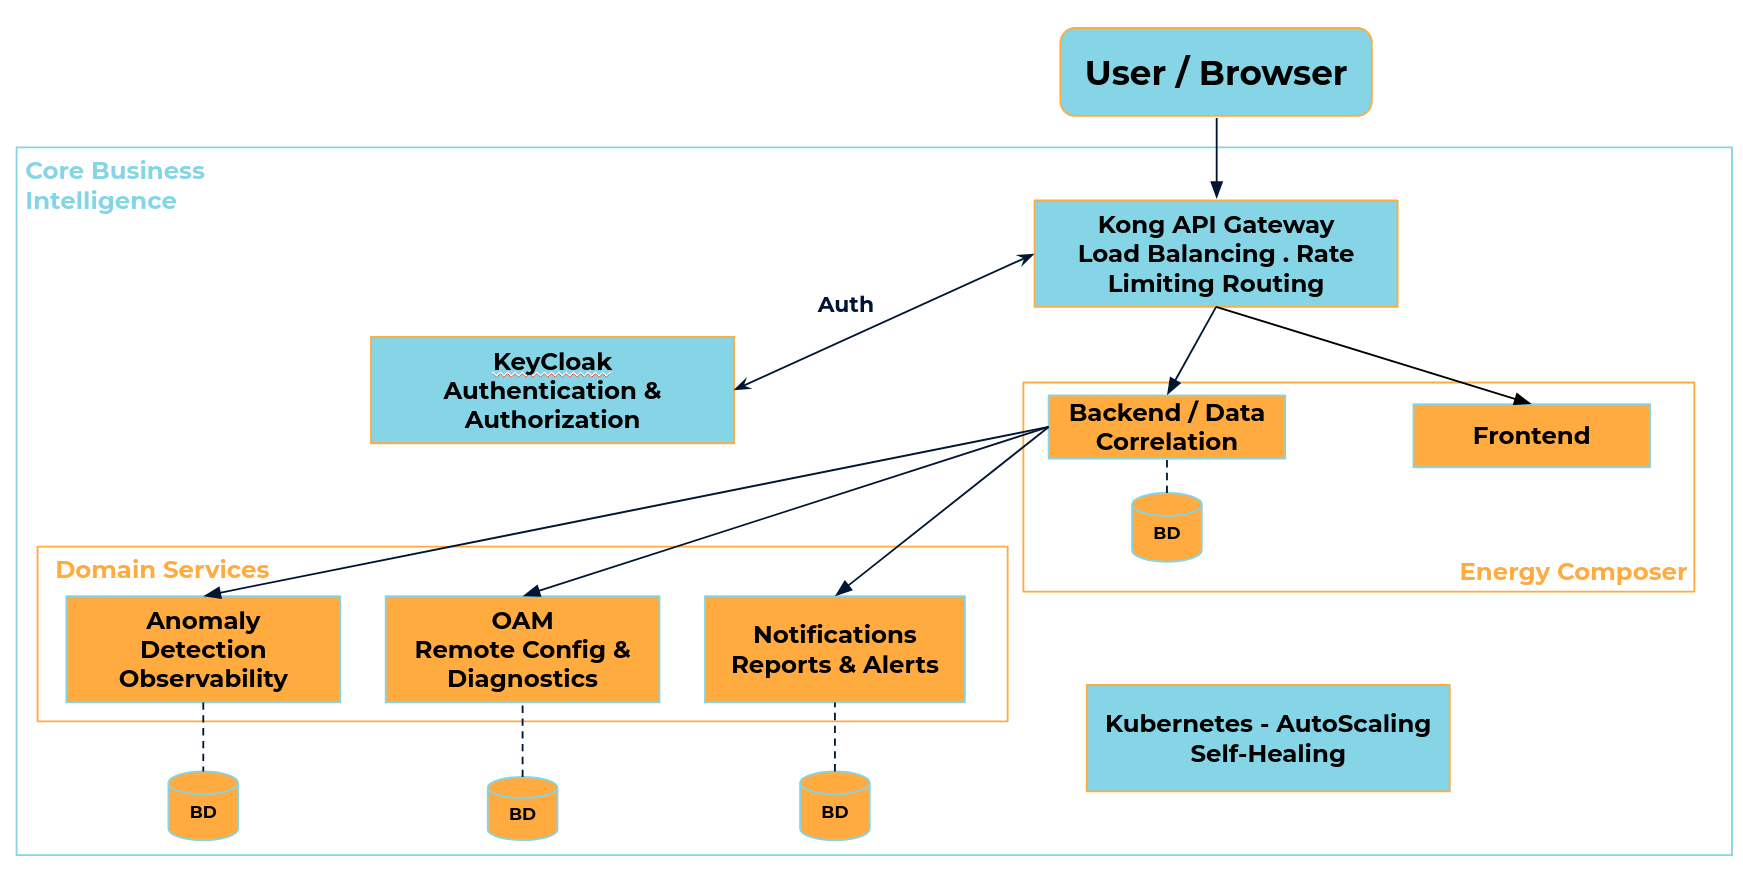
\includegraphics[width=\textwidth]{Diagram.png}
\caption{VoltGuard high-level architecture.}
\label{fig:architecture}
\end{figure}

\section{Technology Choices}


\begin{table}[H]
\centering
\caption{Technology stack per service}
\label{tab:tech}
\renewcommand{\arraystretch}{1.3}
\begin{tabularx}{\textwidth}{l l X}
\toprule
\textbf{Component} & \textbf{Stack} & \textbf{Rationale} \\
\midrule
Composer Frontend  & React + Vite       & Component-driven SPA with fast HMR for development \\
Composer Backend   & Node.js / Express  & Lightweight SOA gateway; rich ecosystem for HTTP proxying \\
OAM Service          & Rust / Axum / SQLx & Memory safety and throughput for sensor inventory operations \\
Anomaly Detection    & Python / FastAPI   & Native ecosystem for ML libraries (Prophet) \\
Notifications        & Python / Connexion & OpenAPI-first design enforced by the Connexion framework \\
API Gateway          & Kong 3.7 (DB-less) & Declarative config, zero-DB overhead, native K8s support \\
Authentication       & Keycloak 25        & Standards-compliant OIDC with PKCE; battle-tested in production \\
Observability        & Prometheus + Grafana & De facto standard for cloud-native metrics collection and visualisation \\
Orchestration        & Kubernetes         & Self-healing pods, HPA, declarative infrastructure-as-code \\
\bottomrule
\end{tabularx}
\end{table}

\section{Communication Patterns}

\begin{itemize}[noitemsep]
  \item \textbf{Client → Kong}: HTTPS termination at the university Ingress Controller; Kong receives plain HTTP on port 8000.
  \item \textbf{Kong → Services}: Internal Kubernetes DNS.
  \item \textbf{Composer Backend → Peers}: Proxied REST calls with configurable timeout, retry count, and backoff.
  \item \textbf{Anomaly → Notifications}: Direct internal HTTP POST when an anomaly is confirmed.
  \item \textbf{Prometheus → Services}: Pull-based scrape every 15 seconds against each service's \texttt{/metrics} endpoint.
\end{itemize}

% ============================================================
\chapter{Composer Service}
\label{ch:composer}
% ============================================================

\section{Overview}

The Composer Service is the user-facing core of VoltGuard. It consists of two sub-components: a \textbf{React frontend} that provides the operator dashboard, and a \textbf{Node.js backend} that acts as a Service-Oriented Architecture (SOA) gateway — aggregating and normalising data from all peer microservices before presenting it to the client.

\section{Frontend}

\subsection{Technology \& Build}

The frontend is built with \textbf{React 18} and \textbf{Vite}, served as a static Single-Page Application from an nginx container. Authentication is handled client-side using \textbf{Keycloak-js} with the PKCE flow, which requires a secure context (HTTPS or localhost). The Keycloak URL is injected at build time via a Vite environment variable:

\begin{lstlisting}[language=bash, caption=Frontend Docker build arguments]
docker build \
  --build-arg VITE_AUTH_DISABLED=false \
  --build-arg VITE_KEYCLOAK_URL=https://grupo4-egs-deti.ua.pt/auth \
  -t registry.deti/grupo4-egs-deti.ua.pt/compositor-frontend:v5 \
  composer-service/frontend/
\end{lstlisting}

\subsection{Key Design Decisions}

\begin{itemize}[noitemsep]
  \item Authentication variables are \textbf{build-time} (baked into the JS bundle), not runtime — this is a Vite constraint; \texttt{VITE\_*} vars are resolved at \texttt{npm run build}.
  \item The nginx configuration sets \texttt{expires 1y; Cache-Control: public, immutable} for all static assets (JS, CSS, PNG), which maximises caching efficiency for content-hashed filenames.
  \item \texttt{VITE\_AUTH\_DISABLED} is independent of the backend's \texttt{AUTH\_DISABLED} — both must be consistent or API calls will fail with 403.
\end{itemize}

\section{Backend}

\subsection{Technology \& Role}

The backend is a \textbf{Node.js / Express} API that acts as the single integration point for all data consumers. It does not own any domain data directly; instead, it proxies and aggregates requests to OAM, Anomaly Detection, and Notifications.

\subsection{Security}

All endpoints are protected by Keycloak JWT validation. The backend verifies tokens against the Keycloak realm and rejects unauthenticated requests with HTTP 401. Sensitive configuration (client secrets, session keys, auth tokens) is loaded from Kubernetes secrets at runtime, never from plain environment variables in the deployment manifest.

% ============================================================
\chapter{OAM Service}
\label{ch:oam}
% ============================================================

\section{Overview}

The \textbf{Operations, Administration and Maintenance (OAM)} service manages the lifecycle of physical sensors deployed in the field. It is responsible for sensor registration, firmware inventory, and keepalive tracking.

\section{Technology}

The OAM service is written in \textbf{Rust} using the \textbf{Axum} web framework, with \textbf{SQLx} for async PostgreSQL access. Rust was chosen for its memory safety guarantees and predictable latency under load, important properties for a service that receives frequent keepalive heartbeats from a large sensor fleet.

\section{Data Model}

The service uses a \textbf{PostgreSQL 17} database managed by SQLx migrations. Persistent state includes:

\begin{itemize}[noitemsep]
  \item \textbf{Sensors} — unique identifier, location (district), firmware version, last-seen timestamp.
  \item \textbf{Firmware} — binary blobs stored on a persistent volume, with version metadata and checksum.
  \item \textbf{Keepalives} — timestamped heartbeat records used to detect sensor offline events.
\end{itemize}

\section{API Surface}

The OAM service exposes a REST API documented via OpenAPI (Swagger UI at \texttt{/swagger-ui}). Key endpoint groups:

\begin{table}[H]
\centering
\caption{OAM service endpoint groups}
\label{tab:oam-endpoints}
\renewcommand{\arraystretch}{1.3}
\begin{tabular}{l l l}
\toprule
\textbf{Group} & \textbf{Path prefix} & \textbf{Description} \\
\midrule
Sensors     & \texttt{/sensors}      & CRUD for sensor registry \\
Firmware    & \texttt{/firmware}     & Upload, list, and assign firmware versions \\
Keepalive   & \texttt{/keepalive}    & Sensor heartbeat endpoint \\
\bottomrule
\end{tabular}
\end{table}

\section{Kubernetes Storage}

Two PersistentVolumeClaims back the OAM service:

\begin{itemize}[noitemsep]
  \item \texttt{oam-postgres-data}  — PostgreSQL data directory.
  \item \texttt{oam-firmware-storage}  — Firmware binary blobs.
\end{itemize}

% ============================================================
\chapter{Anomaly Detection Service}
\label{ch:anomaly}
% ============================================================

\section{Overview}

The Anomaly Detection service is the intelligence layer of VoltGuard. It ingests sensor readings, models the expected baseline for each sensor, and flags readings that deviate significantly from that baseline.

\section{Machine Learning Pipeline}

The pipeline uses a robust time-series forecasting approach:

\begin{itemize}
  \item \textbf{Prophet} (Meta / Facebook) - a decomposable time-series forecasting model that captures trend and seasonality. The pipeline splits incoming datasets using an \textbf{80/20 rule}: 80\% of the historical data is used to train the model and establish the baseline, while the remaining 20\% is then used for validation and \textbf{historical anomaly detection}, where any readings falling outside the generated confidence interval are flagged.
\end{itemize}

A reading is escalated to the Notifications service only if it falls outside the established Prophet confidence interval, ensuring proactive anomaly detection.

\section{Future Forecasting}

Beyond historical analysis, the persisted Prophet model unlocks proactive capabilities. The System can generate on-demand \textbf{forecasts} to project future energy consumption. This allows facility managers to anticipate energy spikes and plan accordingly, shifting the platform from a purely reactive monitor to a proactive intelligence tool.

\section{Dynamic Calibration}

Voltguard exposes configurable parameters to system operators. Through the frontend dashboard, users can dynamically adjust the \textbf{Prophet uncertainty interval}.

\section{API}

The service is built with \textbf{FastAPI} and exposes:

\begin{itemize}[noitemsep]
  \item \texttt{GET /measurements} — retrieves historical sensor readings.
  \item \texttt{GET /anomalies} — query confirmed anomaly events.
  \item \texttt{GET /forecasts/\{sensor\_id\}} — generate future consumption forecasts on-demand using the persisted model.
  \item \texttt{PUT /models/\{model\_id\}/config} — update the model sensitivity and configuration parameters.
  \item \texttt{POST /webhooks} — register an endpoint for asynchronous processing callbacks.
  \item \texttt{GET /metrics} — Prometheus metrics endpoint.
  \item \texttt{GET /docs} — auto-generated FastAPI interactive documentation.
\end{itemize}

\section{Secrets \& Configuration}

The service uses a \texttt{vault\_loader.py} module to pull sensitive configuration (such as the \texttt{ANOMALY\_APP\_TOKEN}) from HashiCorp Vault at startup. In the Kubernetes deployment, Vault is replaced by Kubernetes Secrets injected as environment variables.

% ============================================================
\chapter{Notifications Service}
\label{ch:notifications}
% ============================================================

\section{Overview}
The Notifications service is a multi-channel alerting gateway that acts as an abstraction layer for operational communications. When the system's orchestrator (Composer) detects an anomaly event, it actively invokes this service by dispatching an HTTP \texttt{POST} request containing the payload. Upon receiving the request, the Notifications service evaluates user-defined routing profiles and executes the delivery process accordingly.

\section{Technology Stack}
The Notifications service is built upon a modern, asynchronous pythonic ecosystem designed for high throughput and strict contract enforcement. The complete technology stack comprises the following components:

\begin{itemize}
    \item \textbf{Framework \& API Enforcement:} Follows an \textbf{OpenAPI-first} approach using \textbf{Connexion}, a Python framework that dynamically generates the WSGI application layer.
    \item \textbf{Email Dispatch:} Implements native \textbf{SMTP} protocols through Python's built-in \texttt{smtplib} and \texttt{email} packages, supporting secure \textbf{TLS} encryption and integration with modern relay providers (e.g., Gmail App Passwords).
    \item \textbf{SMS Gateway:} Leverages the external \textbf{Twilio REST API} via the official \texttt{twilio} client library for transactional and operational mobile text messaging.
    \item \textbf{Extensible Architecture:} The core dispatch motor is decoupled from hardcoded credentials, dynamically consuming provider parameters from the database to allow seamless runtime registration or over-riding of additional communication channels without service downtime.
\end{itemize}

\section{Stored Data}
The service utilizes a \textbf{MongoDB} database to guarantee loose coupling and dedicated storage. Persistent state includes:
\begin{itemize}
    \item \textbf{User Preferences} — Stores unique user identifiers, cryptographic secrets, channel targets (phone numbers, emails), and alert dispatch policies (immediate vs. digest).
    \item \textbf{Notifications \& Digest Queue} — Holds operational logs of submitted payloads and a dedicated buffer queue for deferred alert aggregation.
    \item \textbf{Notification Audit} — Keeps a structured lifecycle event trail (e.g., \texttt{CREATED}, \texttt{DELIVERY\_ATTEMPT}, \texttt{ABORTED\_BY\_PREFERENCE}) for diagnostic and compliance purposes .
\end{itemize}

\section{Supported Channels and API Features}
All channel integrations are decoupled from core business logic, supporting native email transmission and SMS integrations. Delivery is protected by an idempotency layer.

\begin{table}[h!]
\centering
\caption{Supported notification channels}
\label{tab:supported_channels}
\begin{tabular}{ll}
\hline
\textbf{Channel} & \textbf{Provider} \\ \hline
Email            & Native SMTP (\texttt{smtplib} with TLS) \\ 
SMS              & Twilio SMS API \\ \hline
\end{tabular}
\end{table}

\begin{itemize}
    \item \textbf{Idempotency Key:} The \texttt{POST /v1/notifications} endpoint enforces an idempotency mechanism using the \texttt{Idempotency-Key} HTTP header to prevent duplicate notifications during network retries.
    \item \textbf{Dynamic Preferences Link:} During the first notification attempt for a specific target, the system dynamically injects an opt-out URL appended with the user's unique cryptographic secret, enabling self-service profile management.
\end{itemize}

% ============================================================
\chapter{Kong API Gateway}
\label{ch:kong}
% ============================================================

\section{Overview}

Kong 3.7 operates in \textbf{DB-less} mode with a declarative configuration (\texttt{kong/kong.yml}). All routing rules, upstream targets, and plugins are defined in that single YAML file, making the gateway configuration fully reproducible and version-controlled.

\section{Routing}

Traffic arrives at the Kong proxy port and is routed to the appropriate upstream service based on the request path. Key routes:

\begin{table}[H]
\centering
\caption{Kong routing table (Kubernetes deployment)}
\label{tab:kong-routes}
\renewcommand{\arraystretch}{1.3}
\begin{tabular}{l l}
\toprule
\textbf{Path / Host pattern} & \textbf{Upstream service} \\
\midrule
\texttt{/}            & Composer Frontend \\
\texttt{/api/*}       & Composer Backend \\
\texttt{/auth/*}      & Keycloak \\
\texttt{/oam/*}       & OAM Service \\
\texttt{/notify/*}    & Notifications Service \\
\texttt{/anomaly/*}   & Anomaly Detection \\
\bottomrule
\end{tabular}
\end{table}

\section{High Availability}

Kong is one of the two components managed by a \textbf{HorizontalPodAutoscaler}. The HPA maintains at least 2 Kong replicas at all times, scaling up to 5 under CPU pressure. This ensures that no single Kong pod failure interrupts service, and that the gateway capacity grows proportionally with incoming traffic.

% ============================================================
\chapter{Deployment \& Infrastructure}
\label{ch:deployment}
% ============================================================

\section{Kubernetes Overview}

All production workloads run in the namespace \texttt{tenant-grupo4-egs-deti-ua-pt} on the DETI cluster. The deployment is fully declarative: applying \texttt{k8s/deployment.yaml} and \texttt{k8s/observability.yaml} brings up the entire platform from scratch.

\subsection{Persistent Volumes}

\begin{table}[H]
\centering
\caption{PersistentVolumeClaims}
\label{tab:pvcs}
\renewcommand{\arraystretch}{1.3}
\begin{tabular}{l l}
\toprule
\textbf{Name} & \textbf{Consumer} \\
\midrule
\texttt{composer-data}        & Composer Backend (session data) \\
\texttt{oam-postgres-data}      & OAM PostgreSQL \\
\texttt{oam-firmware-storage}   & OAM firmware binaries \\
\texttt{notifications-db-data}  & Notifications Service \\
\texttt{keycloak-postgres-data} & Keycloak PostgreSQL \\
\bottomrule
\end{tabular}
\end{table}

\subsection{Secrets}

All sensitive values (database passwords, API tokens, client secrets, session keys) are stored in a Kubernetes Secret resource applied from \texttt{k8s/secrets.yaml} (gitignored). Services consume them as environment variables injected by the kubelet: no secrets ever appear in a container image or deployment manifest.

\section{Load Balancing}

\subsection{Kong as the Single Entry Point}

The university Ingress Controller terminates TLS and forwards all traffic to the Kong Service. Kong then load-balances across its replica pods using the standard Kubernetes Service round-robin mechanism.

\subsection{HorizontalPodAutoscaler}

Two HPAs are configured, both CPU-triggered:

\begin{table}[H]
\centering
\caption{HorizontalPodAutoscaler configuration}
\label{tab:hpa}
\renewcommand{\arraystretch}{1.3}
\begin{tabular}{l c c c}
\toprule
\textbf{Component} & \textbf{Min replicas} & \textbf{Max replicas} & \textbf{Metric} \\
\midrule
Kong Gateway         & 2 & 5 & CPU utilisation \\
Composer Frontend  & 2 & 5 & CPU utilisation \\
\bottomrule
\end{tabular}
\end{table}

The minimum of 2 replicas for both components ensures that a single pod failure never causes a service outage, so there is always at least one healthy pod handling requests while Kubernetes reschedules the failed one.

\section{Observability}

The observability stack is deployed via \texttt{k8s/observability.yaml} and consists of:

\begin{itemize}[noitemsep]
  \item \textbf{Prometheus} (\texttt{prom/prometheus:v2.53.1}) — scrapes all application services every 15 seconds.
  \item \textbf{Grafana} (\texttt{grafana/grafana:11.1.0}) — serves pre-provisioned dashboards at \texttt{/grafana}.
\end{itemize}

\begin{table}[H]
\centering
\caption{Prometheus scrape targets}
\label{tab:prometheus}
\renewcommand{\arraystretch}{1.3}
\begin{tabular}{l l}
\toprule
\textbf{Job name} & \textbf{Metrics path} \\
\midrule
\texttt{anomaly-api}          & \texttt{anomaly-api:8085/metrics} \\
\texttt{composer-backend}   & \texttt{compositor-backend:8080/metrics} \\
\texttt{notifications-service}& \texttt{notifications-service:8083/metrics} \\
\texttt{oam-service}          & \texttt{oam-service:8080/metrics} \\
\bottomrule
\end{tabular}
\end{table}

\section{Stress Testing}

Load testing was performed from a local machine using Apache Bench (\texttt{ab}) against the public HTTP endpoint:

\begin{lstlisting}[language=bash, caption=Stress test command]
ab -n 100000 -c 200 http://grupo4-egs-deti.ua.pt/
\end{lstlisting}

This generates 100,000 requests with a concurrency of 200. Under this load:

\begin{itemize}[noitemsep]
  \item The HPA scales Kong and Frontend pods up from 2 toward the 5-replica ceiling.
  \item Prometheus captures the CPU utilisation spike.
  \item Grafana dashboards provide real-time visibility into request rates and pod behaviour.
  \item Kong handles the burst with negligible connection failures.
\end{itemize}

Scaling events can be monitored live:

\begin{lstlisting}[language=bash, caption=Monitor HPA scaling events]
kubectl get hpa -n tenant-grupo4-egs-deti-ua-pt --watch
\end{lstlisting}

\begin{figure}[H]
\centering

\includegraphics[width=\textwidth]{stress_Requests.png}
\caption{ApacheBench executing 100,000 requests at concurrency 200 against the live cluster — 99,978 requests completed.}
\label{fig:stress-requests}
\end{figure}

\begin{figure}[H]
\centering

\includegraphics[width=\textwidth]{Creating_pods.png}
\caption{Kong CPU at 393\% and Frontend at 359\% of target — new pods enter \texttt{ContainerCreating} state as the HPA responds to the spike.}
\label{fig:creating-pods}
\end{figure}

\begin{figure}[H]
\centering

\includegraphics[width=\textwidth]{logs_pods.png}
\caption{HPA event stream: both HPAs scale up to 5 replicas under load, then step back down to 2--4 as CPU drops below target.}
\label{fig:hpa-events}
\end{figure}

\section{Resilience Testing}

To validate that the platform tolerates pod failures during live traffic, a resilience test was performed with simultaneous pod termination under load.

\subsection{Procedure}

\textbf{Terminal 1 — apply sustained load:}
\begin{lstlisting}[language=bash, caption=Resilience test load]
ab -n 5000 -c 50 http://grupo4-egs-deti.ua.pt/
\end{lstlisting}

\textbf{Terminal 2 — watch pod states and kill a Frontend pod:}
\begin{lstlisting}[language=bash, caption=Watch pod lifecycle and simulate pod failure]
# Watch pod state changes in real time
kubectl get pods -n tenant-grupo4-egs-deti-ua-pt --watch

# In the same or a separate pane: terminate a Frontend pod
kubectl delete pod <composer-frontend-pod-name> -n tenant-grupo4-egs-deti-ua-pt
\end{lstlisting}

\subsection{Observed Behaviour}

Upon pod deletion:

\begin{enumerate}[noitemsep]
  \item The deleted pod transitions to \texttt{Terminating}.
  \item Kubernetes immediately begins scheduling a replacement pod (\texttt{ContainerCreating}).
  \item The surviving Frontend replica continues serving requests.
  \item The replacement pod reaches \texttt{Running} within approximately 10--20 seconds.
  \item The HPA re-evaluates and restores the desired replica count.
\end{enumerate}

The \texttt{ab} run completes with zero or negligible failed requests — any failures are limited to connections in-flight at the exact moment of termination — confirming that the platform is resilient to single-pod failures at the gateway layer.

\begin{figure}[H]
\centering
\begin{subfigure}{\textwidth}
  \centering
  
\includegraphics[width=\textwidth]{delete_pods1.png}
  \caption{Initial state: 2 Frontend pods \texttt{Running}; \texttt{kubectl delete pod} command issued.}
  \label{fig:delete1}
\end{subfigure}

\vspace{0.6em}

\begin{subfigure}{\textwidth}
  \centering
  
\includegraphics[width=\textwidth]{delete_pods2.png}
  \caption{Target pod transitions immediately to \texttt{Terminating}; second pod remains \texttt{Running}.}
  \label{fig:delete2}
\end{subfigure}

\vspace{0.6em}

\begin{subfigure}{\textwidth}
  \centering
  
\includegraphics[width=\textwidth]{delete_pods3.png}
  \caption{Replacement pod reaches \texttt{Running} within $\approx$13\,s — cluster restored to 2 healthy replicas.}
  \label{fig:delete3}
\end{subfigure}
\caption{Pod self-healing lifecycle: from deletion through \texttt{Terminating} to a fresh \texttt{Running} replacement.}
\label{fig:resilience}
\end{figure}

% ============================================================
\chapter{Conclusions}
\label{ch:conclusions}
% ============================================================

VoltGuard successfully delivers a production-grade IoT energy monitoring platform within the constraints of a university project. The key achievements are:

\begin{itemize}
  \item \textbf{End-to-end functionality} — from sensor data ingestion, through ML-based anomaly detection, to real-time multi-channel alerting.
  \item \textbf{Resilient deployment} — Kubernetes HPA with a minimum of 2 replicas for both the gateway and the frontend ensures the platform survives pod failures without downtime.
  \item \textbf{Observability} — Prometheus and Grafana provide full visibility into the platform's runtime behaviour, enabling proactive detection of performance degradation.
  \item \textbf{Security} — Keycloak OIDC with PKCE enforces authenticated access; secrets are never stored in version control or container images.
  \item \textbf{Developer experience} — declarative Kubernetes manifests, a local Docker Compose stack for development, and per-service Swagger UIs make the platform accessible to all team members.
\end{itemize}

\end{document}

